%%%%%%%%%%%%%%%%%%%%%%%%%%%%%%%%%%%%%%%%%%%%%%%%%%%%%%%%%%%%%%%

% Set up document

\documentclass{beamer}
\usecolortheme{whale}
\setbeamersize{text margin left=5mm,text margin right=5mm}

% Used to create a section slide between section
\AtBeginSection[]{
  \begin{frame}
  \vfill
  \centering
  \begin{beamercolorbox}[sep=8pt,center,shadow=true,rounded=true]{title}
    \usebeamerfont{title}\insertsectionhead\par%
  \end{beamercolorbox}
  \vfill
  \end{frame}
}

% Remove default navigation symbols and add just  page number
\setbeamertemplate{navigation symbols}{} % Clear default navigation
\addtobeamertemplate{navigation symbols}{}{%
    \usebeamerfont{footline}%
    \usebeamercolor[fg]{footline}%
    \hspace{1em}%
    \insertframenumber/\inserttotalframenumber
}

% CC licence
\usepackage[
    type={CC},
    modifier={by-nc-sa},
    version={3.0},
]{doclicense}

%%%%%%%%%%%%%%%%%%%%%%%%%%%%%%%%%%%%%%%%%%%%%%%%%%%%%%%%%%%%%%%

% Title page

\title{What would other hospitals do with my patient?}
\subtitle{Using explainable machine learning to understand variation in use of clot-busting drugs (\textit{`thrombolysis'}) in stroke}


\author{Kerry Pearn\inst{1}, Anna Laws\inst{1}, Michael Allen\inst{1}, Martin James\inst{2}}

\institute{\inst{1}NIHR South West Peninsula Applied Research Collaboration (ARC)
\inst{2}Royal Devon University Healthcare NHS Foundation Trust}
%\date{March 2023}
\date{}


\begin{document}

%\frame{\titlepage}

\begin{frame}
\titlepage

\end{frame}

%%%%%%%%%%%%%%%%%%%%%%%%%%%%%%%%%%%%%%%%%%%%%%%%%%%%%%%%%%%%%%%

\begin{frame}
\frametitle{Stroke types}

Most stokes (at least four out of five) are caused by a clot in a blood vessel in the brain. This is also called an \emph{ischaemic} stroke.

\vspace{3mm}



\begin{center}
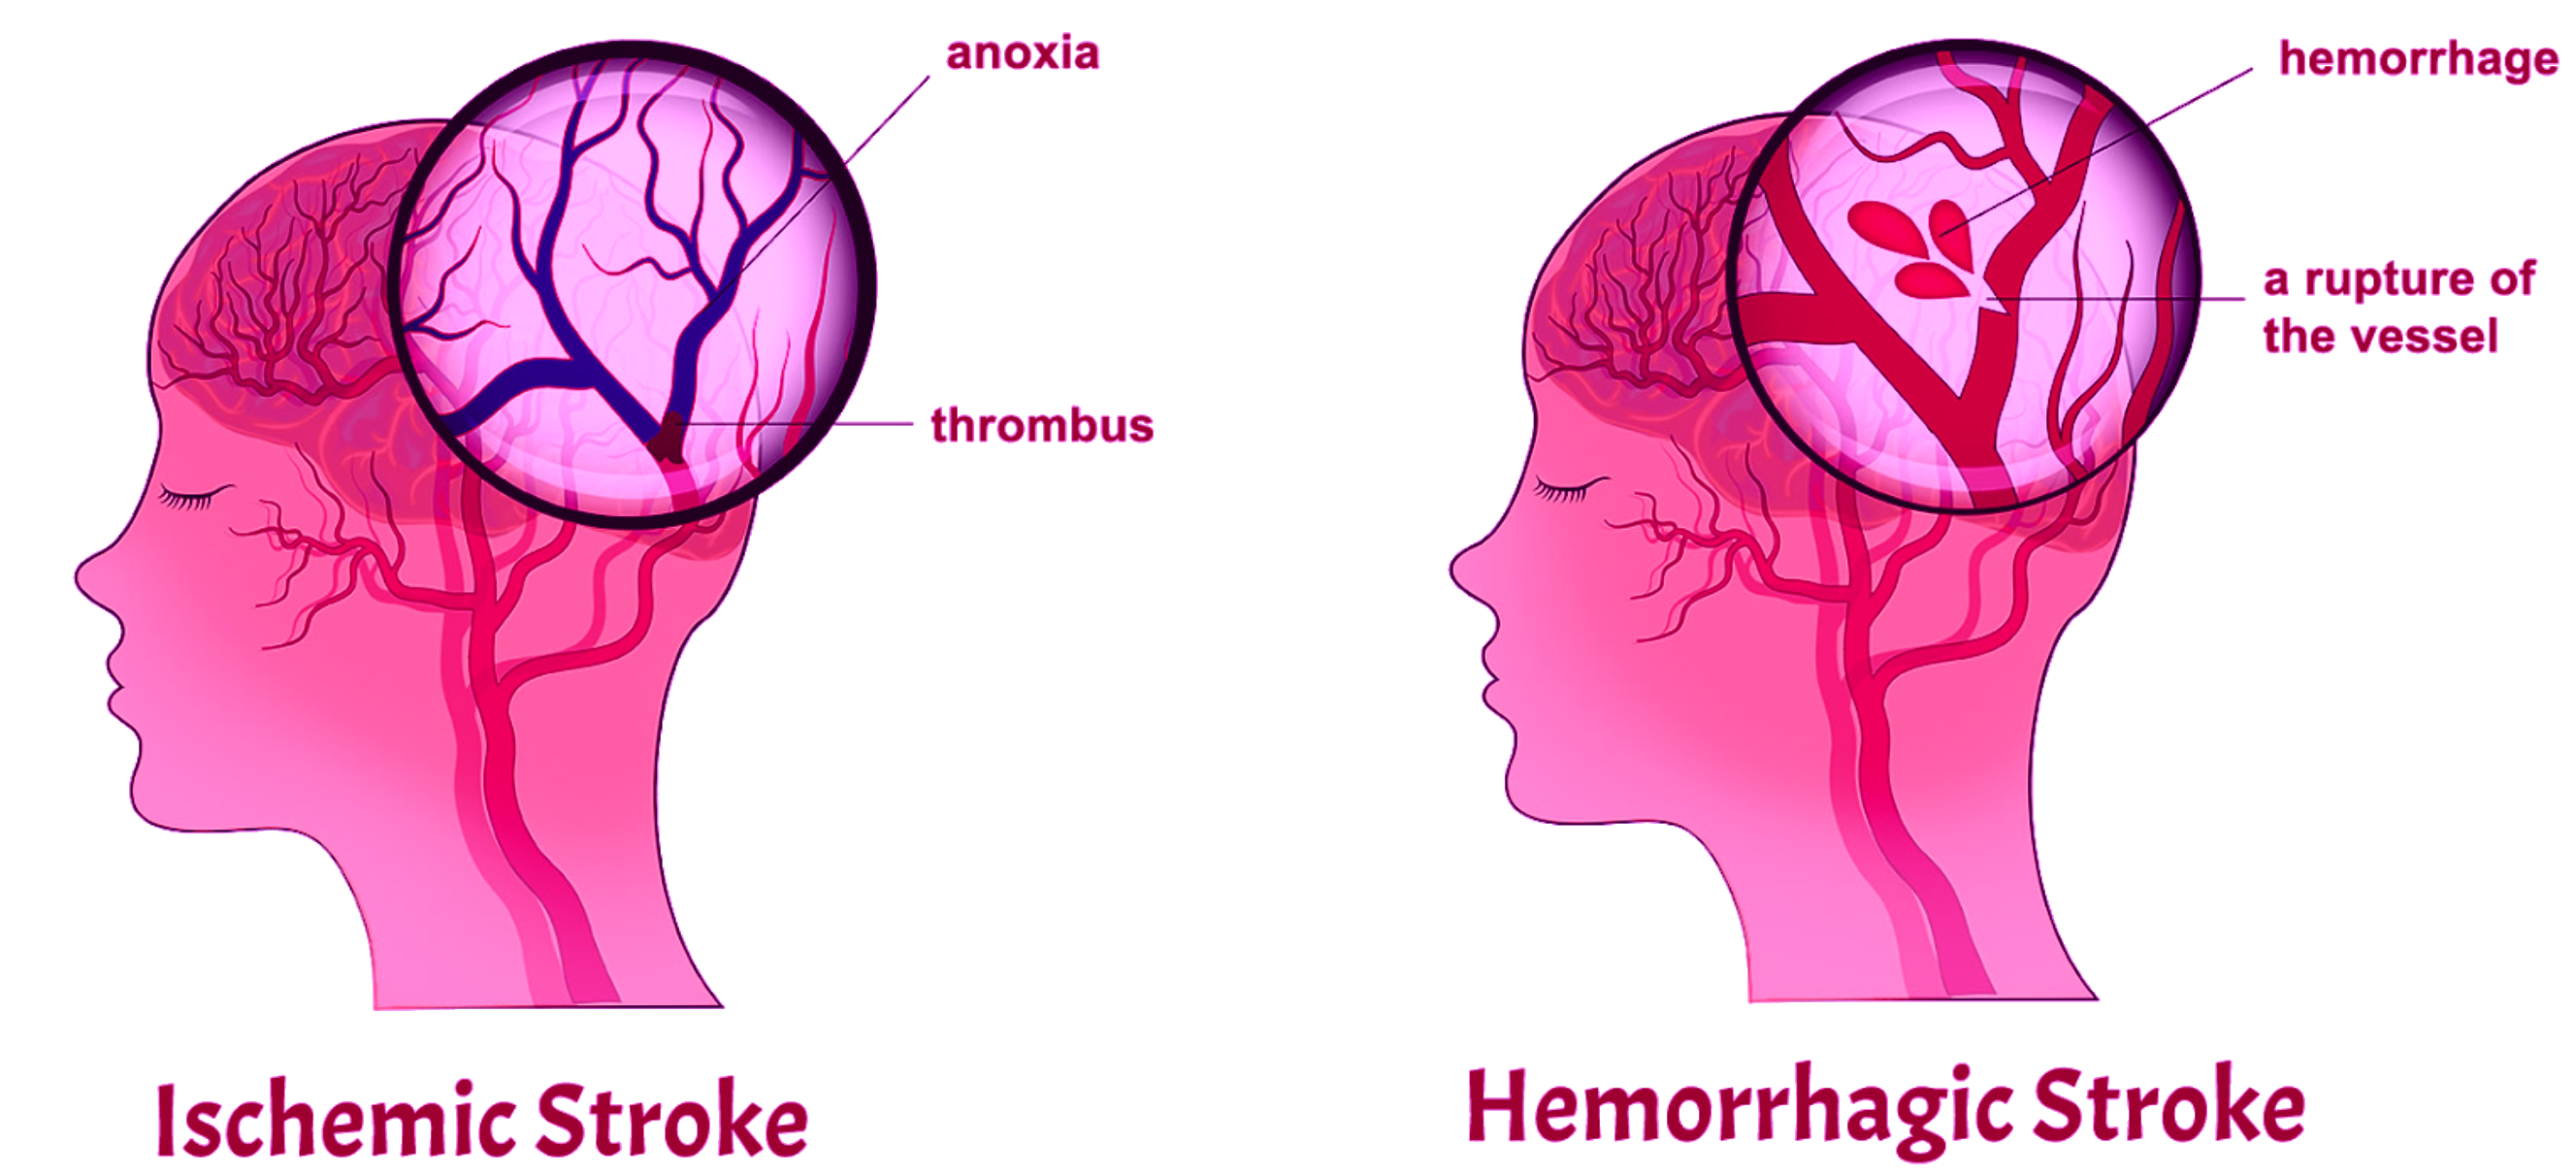
\includegraphics[width=1.0\textwidth]{./images/stroke_types}
\end{center}


\end{frame}
\begin{frame}
\frametitle{Thrombolysis (\emph{'Clot-busting'} medication) in stroke}

While the clot is still fresh, thrombolysis may be given to help break down the clot and restore blood flow.

\vspace{3mm}

\begin{center}
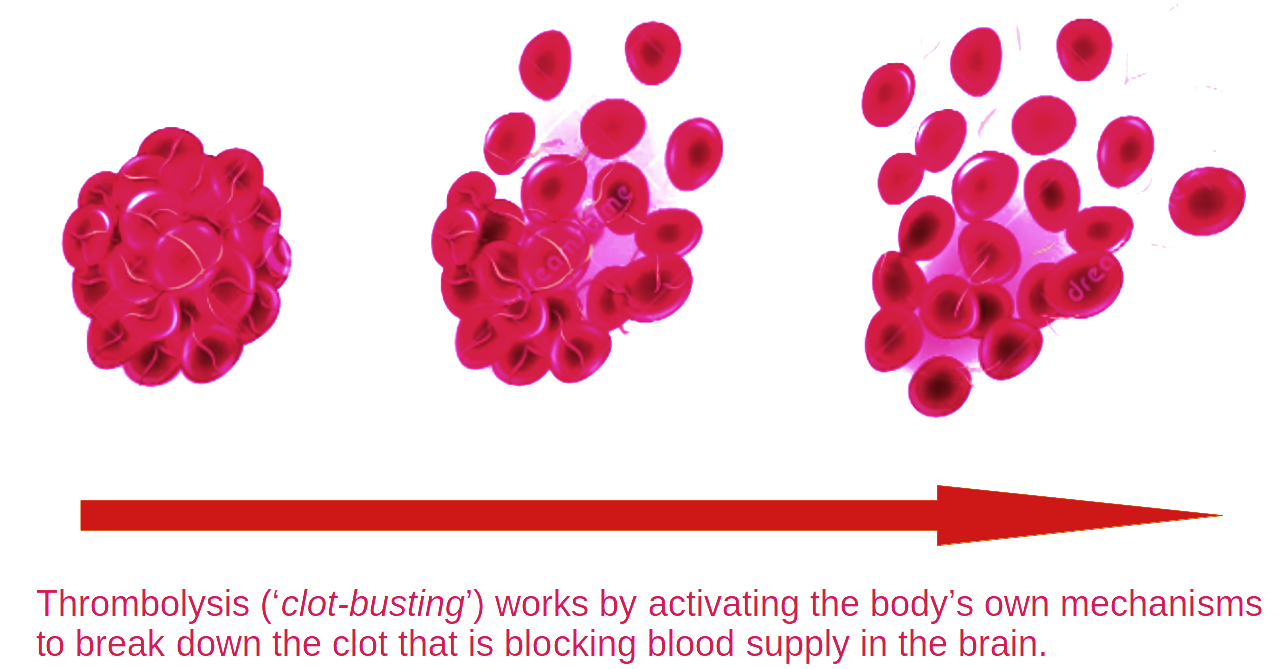
\includegraphics[width=0.70\textwidth]{./images/thrombolysis_mechanism}
\end{center}

\textbf{Drawbacks/limitations}: There is a risk of severe bleed (in about 1 in 50 patients on average, with risk increasing with stroke severity), and thrombolysis loses effectiveness over about the first 5-6 hours.

\end{frame}
\begin{frame}
\frametitle{Use of thrombolysis rates varies significantly between hospitals}

\small
Thrombolysis use varied from below 5\% to 25\% across the 132 acute stroke centres in England and Wales, 2016-2018.
\begin{center}
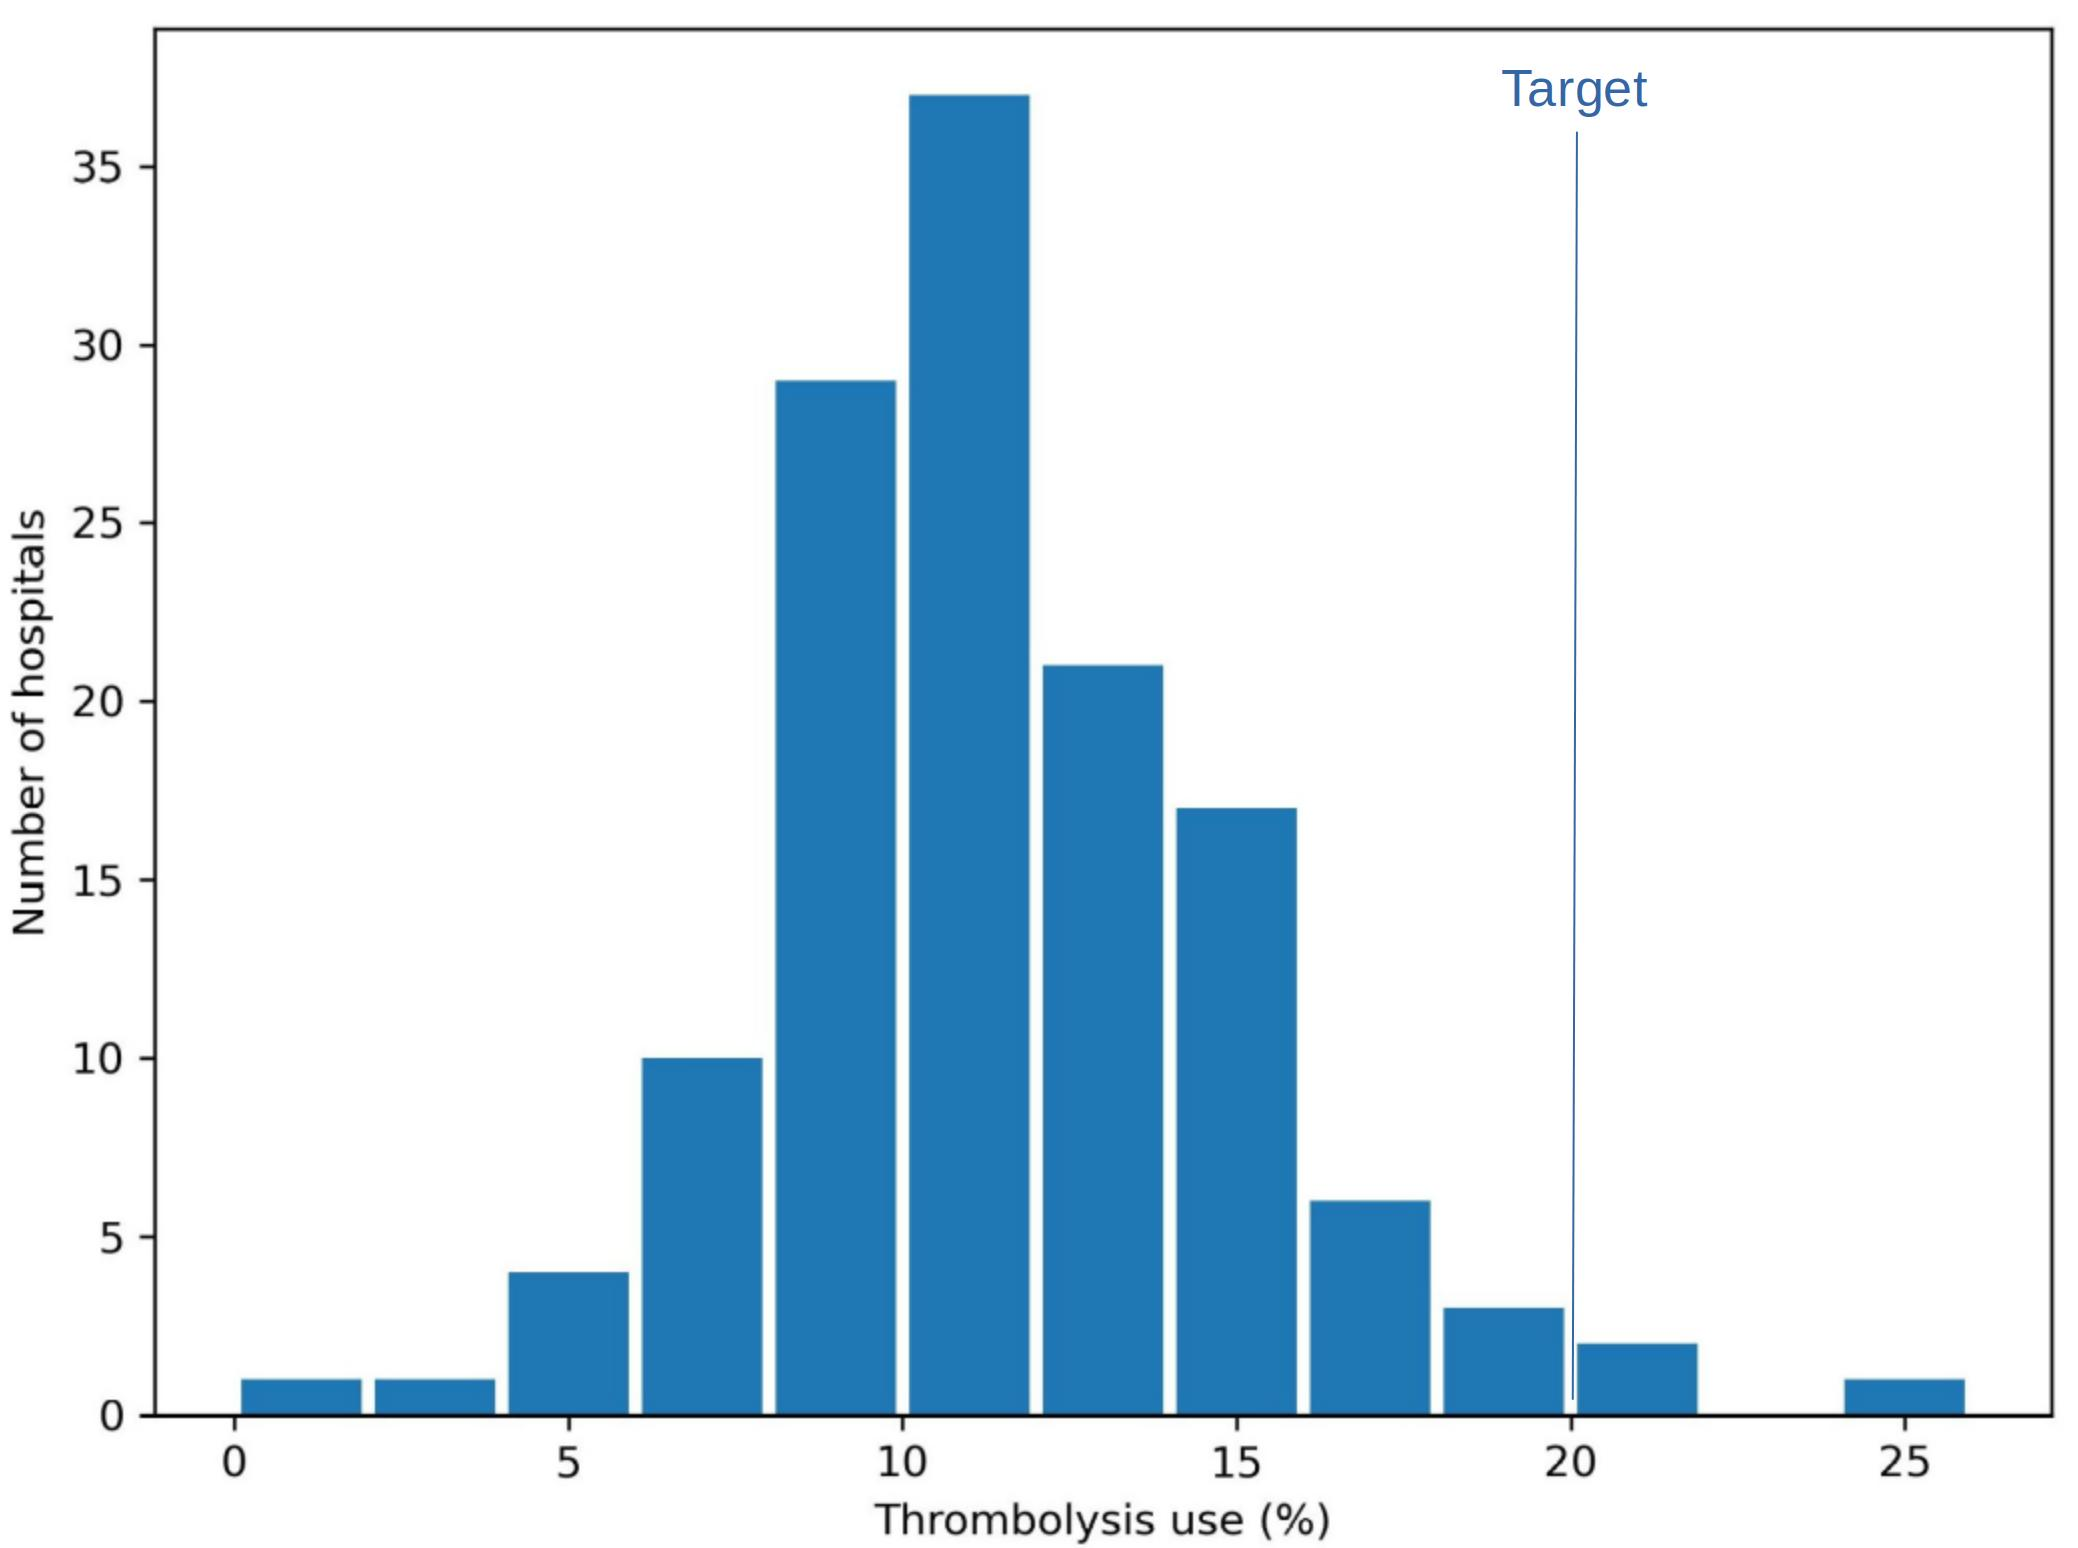
\includegraphics[width=0.50\textwidth]{./images/thrombolysis_by_hospital}
\end{center}

How much of this variation is due to differences in local patient populations, and how much is due to differences in in-hospital processes and decisions hospitals make on who they would give thrombolysis to?
\end{frame}
\begin{frame}
\frametitle{Emgerncey stroke care - what is our problem?}

\begin{center}
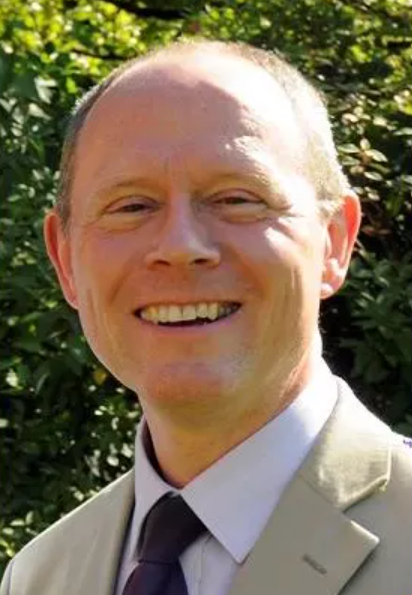
\includegraphics[width=0.27\textwidth]{./images/martin_james}
\\
\small{Prof. Martin James, Clinical Lead of the National Stroke Audit}\\


\vspace{3mm}
\Large
\textit{`Why does use of clot-busting drugs (\textit{`thrombolysis'}) in stroke vary so much?'}

\end{center}   

\end{frame}
\begin{frame}
\frametitle{Can we pickle Martin's brain?}

\begin{center}
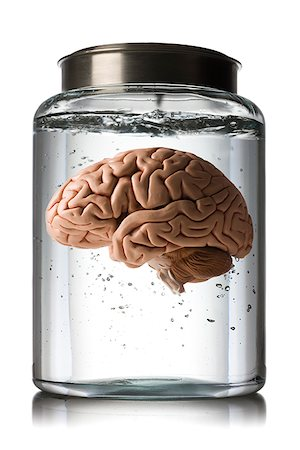
\includegraphics[width=0.40\textwidth]{./images/brain_in_jar}
\\
\small{Can we learn Martin James' expert decision-making on which patients to treat with clot-busting drugs?}
\end{center}   

\end{frame}
\begin{frame}
\frametitle{Can we pickle lots of different brains?}

\begin{center}
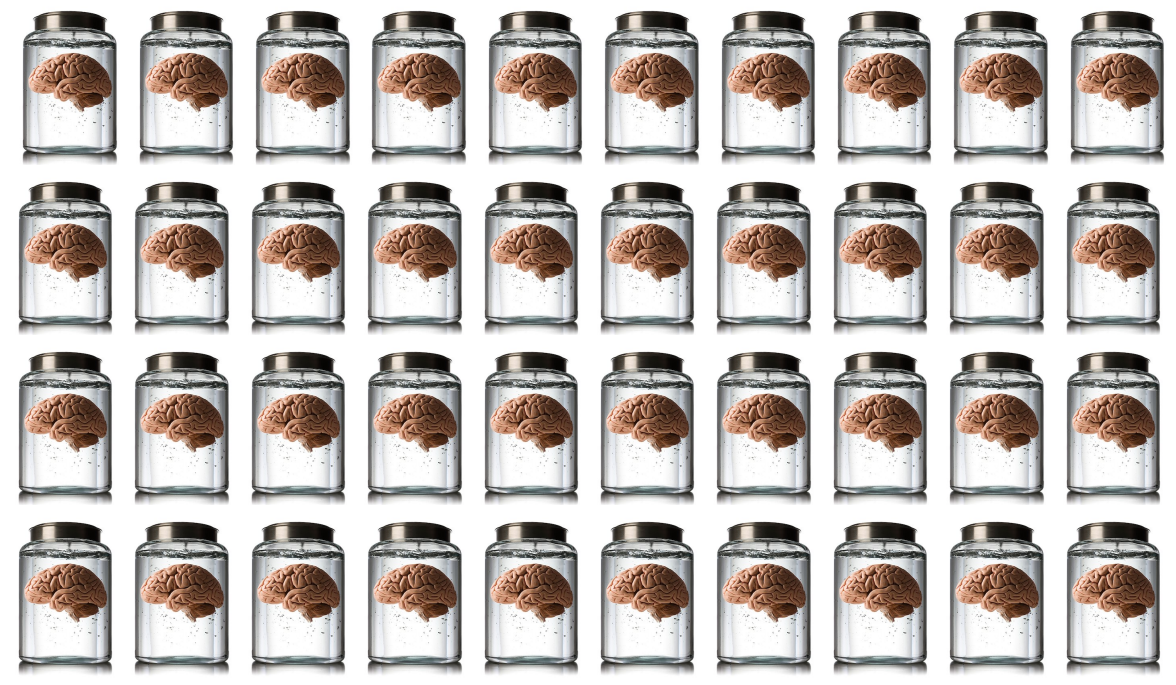
\includegraphics[width=0.9\textwidth]{./images/brains}

\vspace{3mm}
\small{Can we learn lots of different stroke teams' decision-making on which patients to treat with clot-busting drugs?}
\end{center}   

\end{frame}
\begin{frame}
\frametitle{Machine learning overview}
\begin{center}
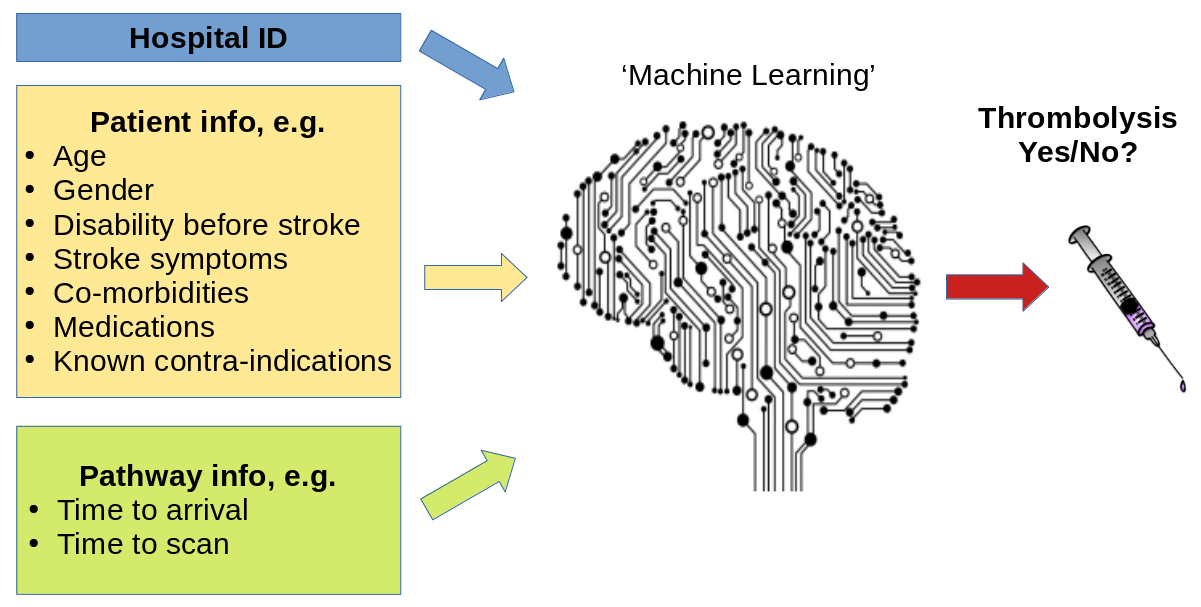
\includegraphics[width=0.80\textwidth]{./images/ml_model_high_level}
\end{center}

\small
\textbf{Machine learning is based on the simple principle of recognising similarity to what has been seen before.}
\vspace{2mm}

\footnotesize{We accessed 246,676 emergency stroke admissions in England and Wales over three years. Our machine learning models use XGBoost classification, and are based on those 88,928 patients who arrive within 4 hours of known stroke onset. Accuracy = 85\% (ROC AUC = 0.92).}
\end{frame}
\begin{frame}
\frametitle{Can we dissect our pickled brains?}

\begin{center}
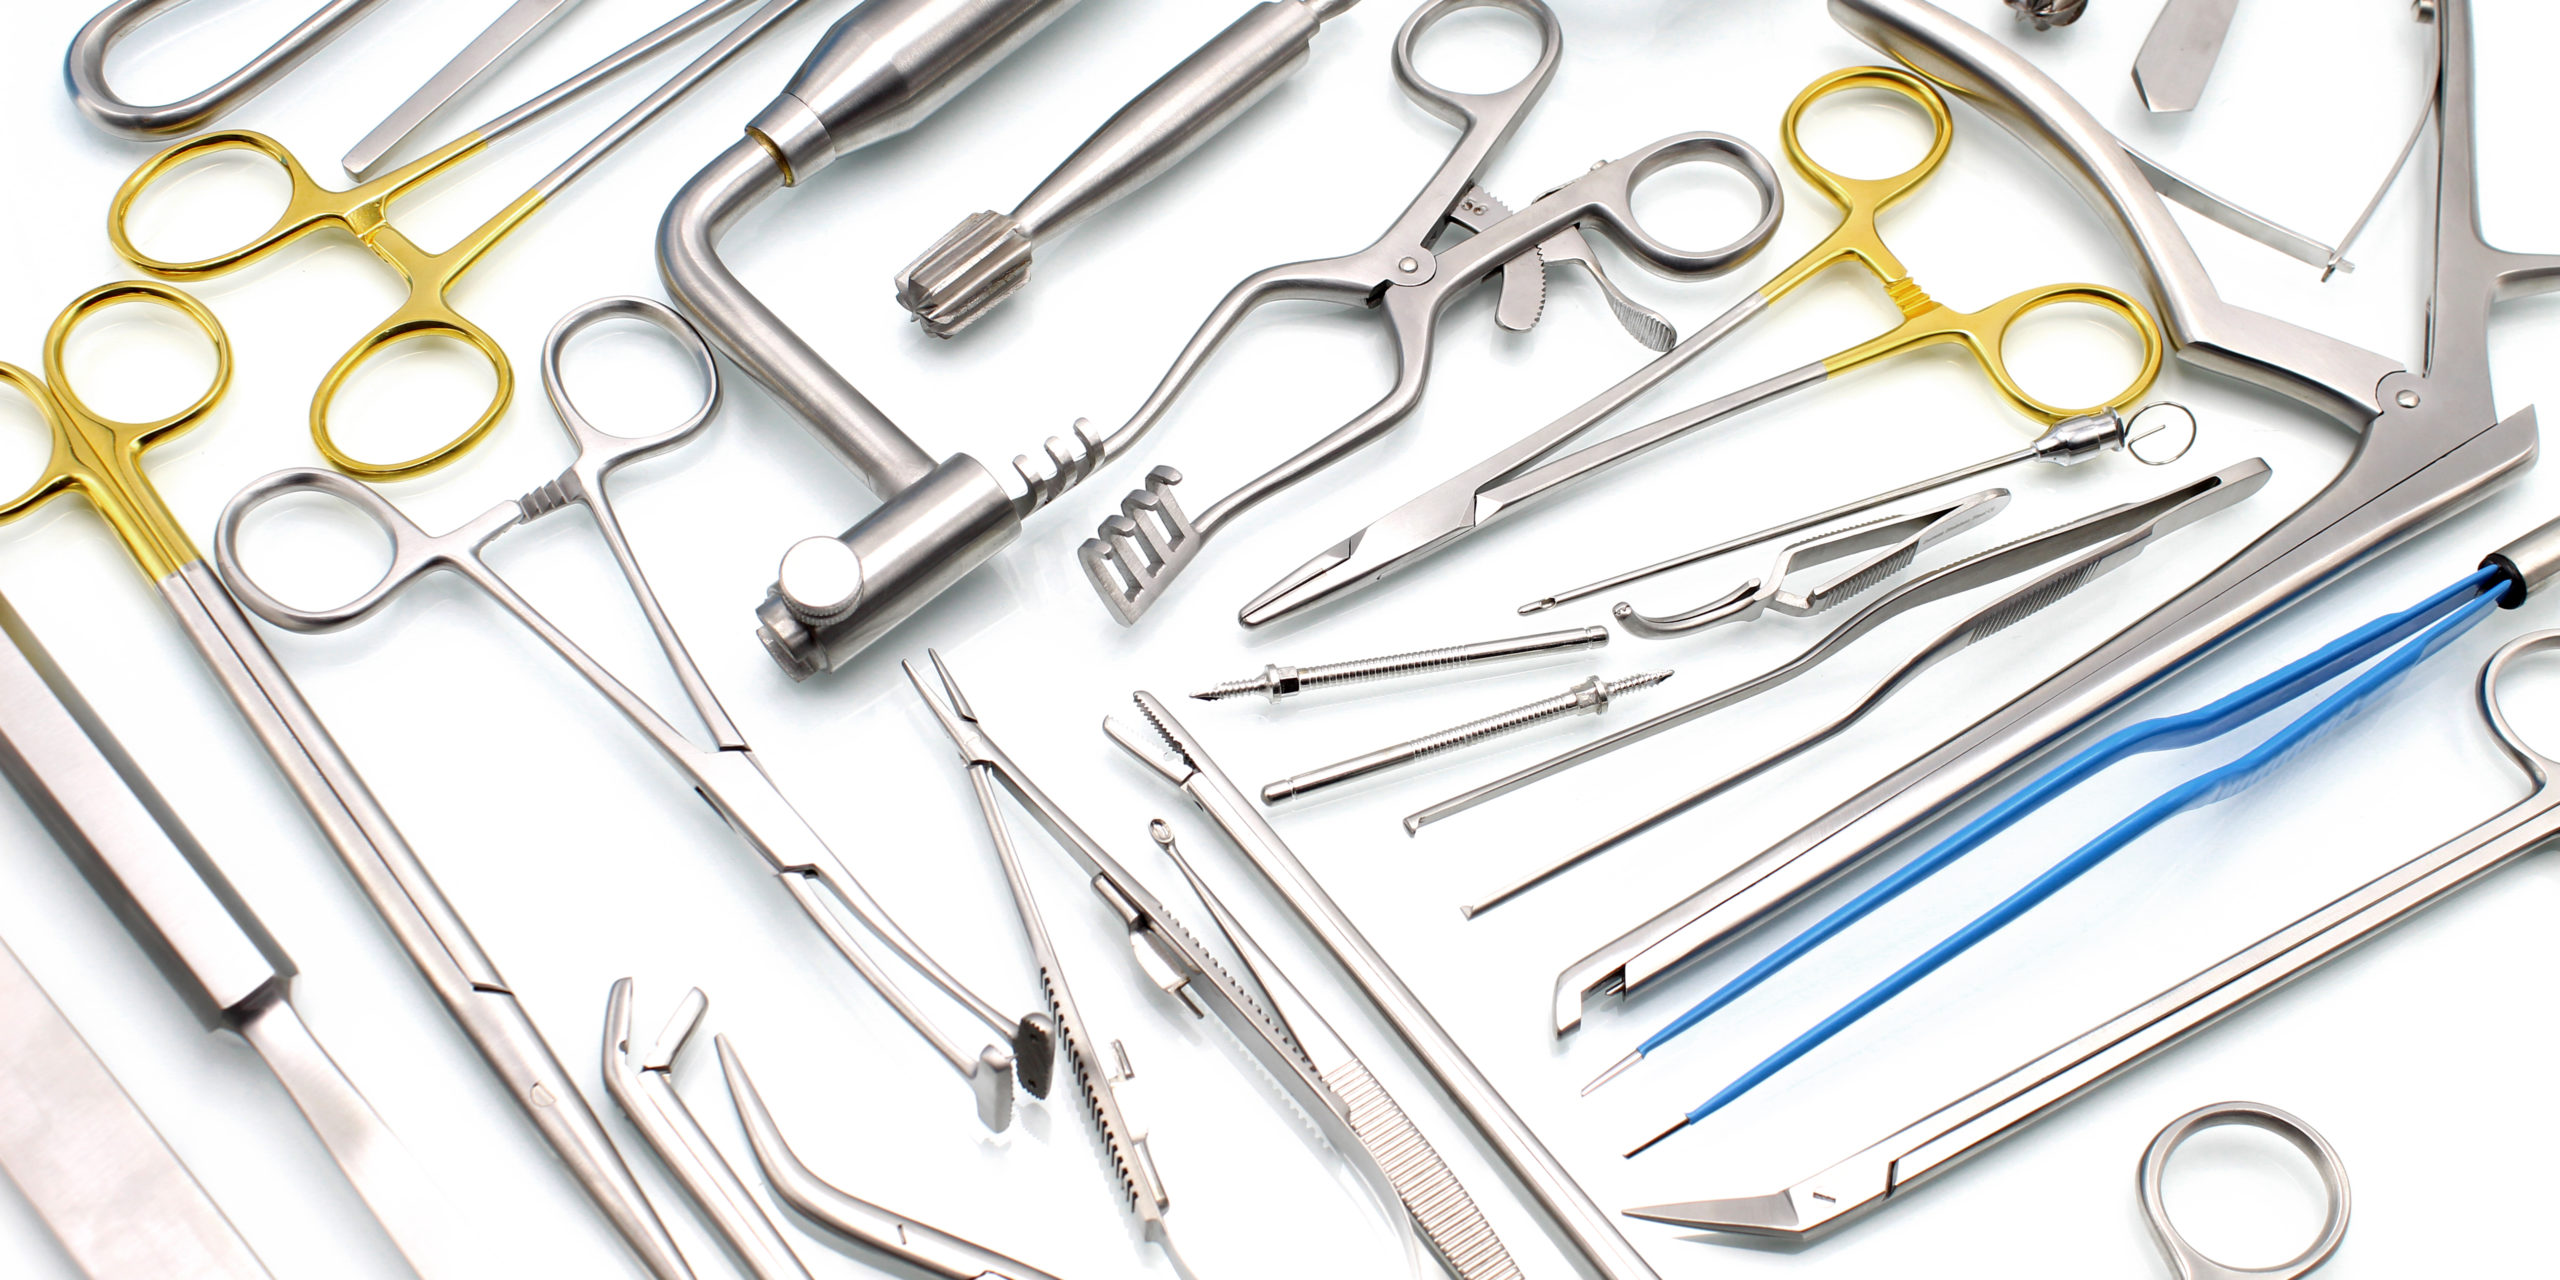
\includegraphics[width=0.9\textwidth]{./images/surgical_instruments}
\\
\vspace{3mm}
\small{Can we uncover what is the same and different between the different decision-making models?}
\end{center}   

\end{frame}
\begin{frame}
\frametitle{SHAP values example}
\begin{center}
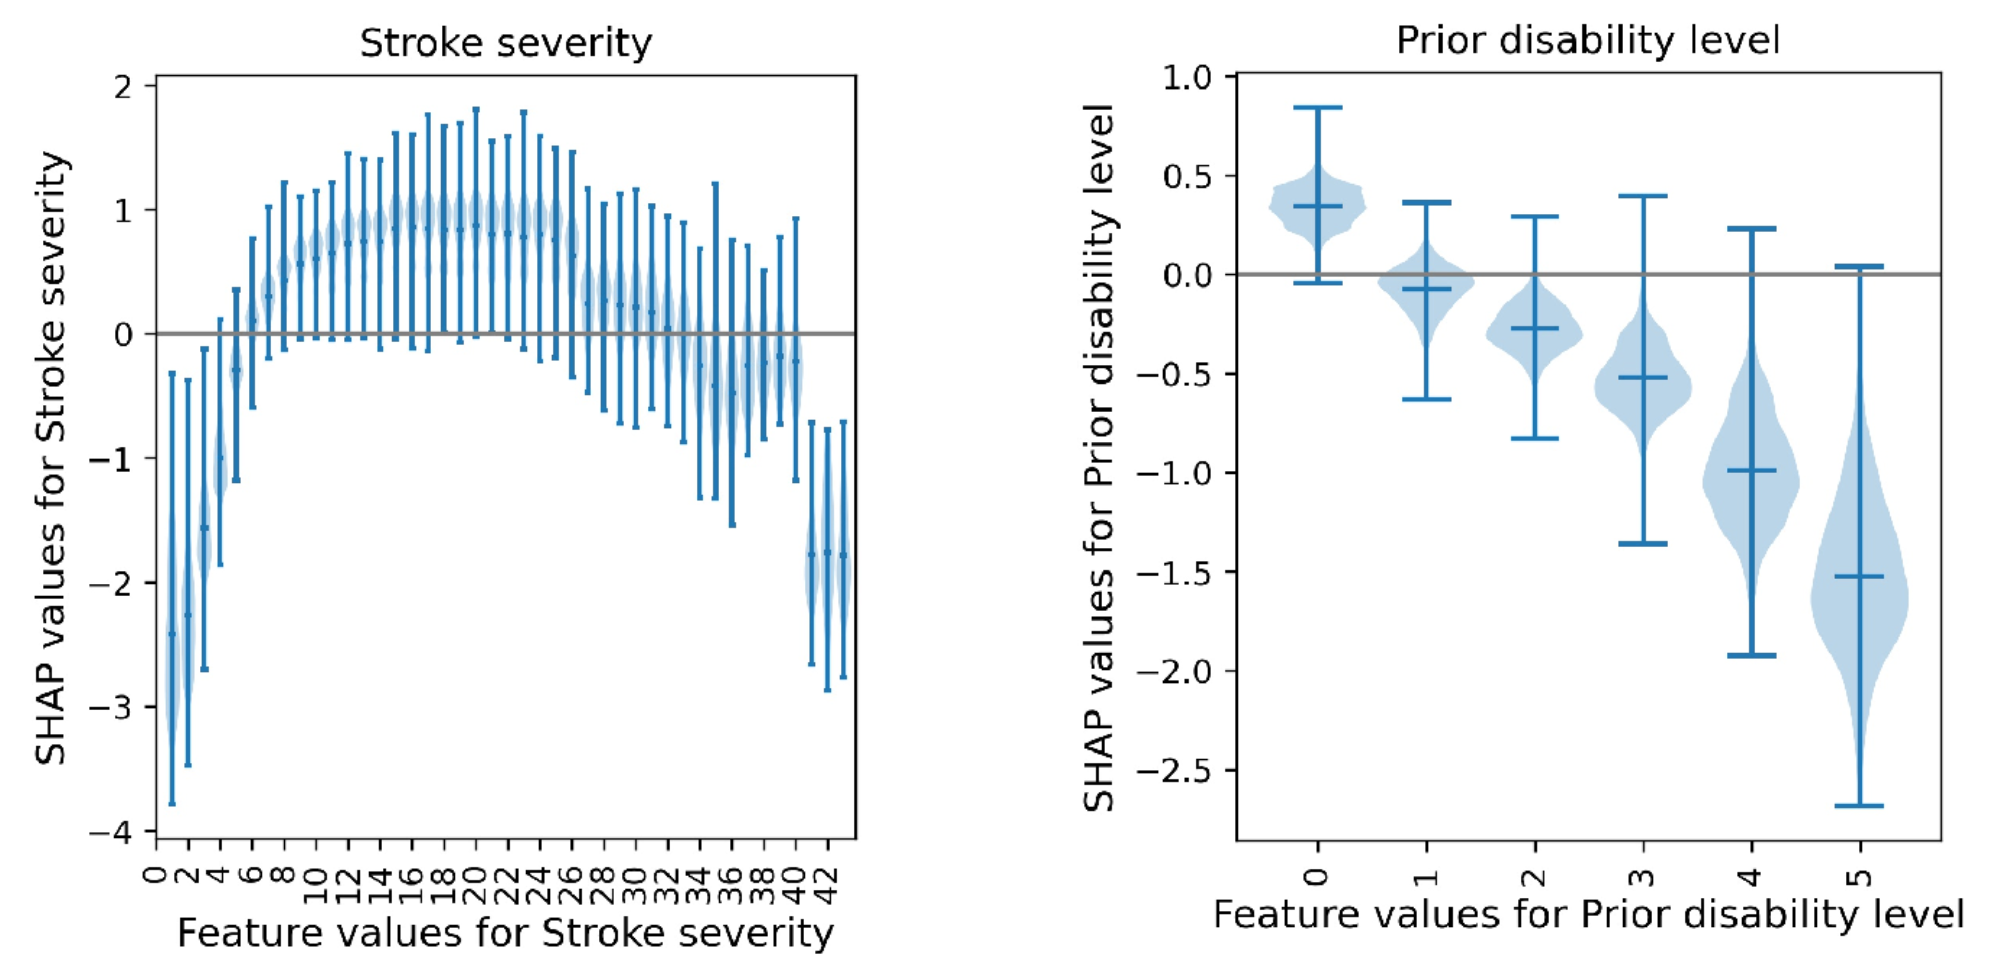
\includegraphics[width=1.0\textwidth]{./images/shap_example}
\end{center}
\end{frame}
\begin{frame}
\frametitle{A proposed model of variation in thrombolysis use}

\begin{center}
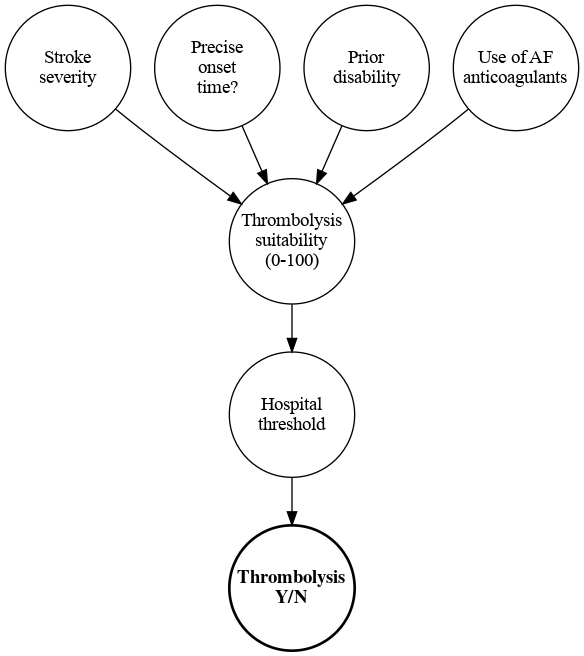
\includegraphics[width=0.55\textwidth]{./images/thrombolysis_causal}
\end{center}   

\end{frame}
\begin{frame}
\frametitle{What if my patient attended a different hospital?}
\begin{center}
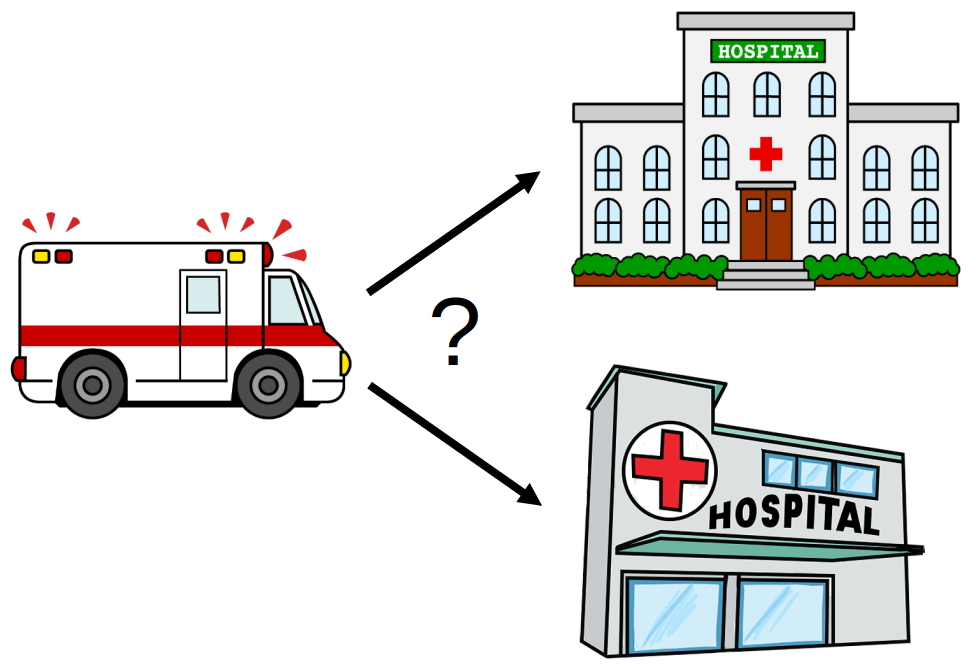
\includegraphics[width=0.60\textwidth]{./images/two_hopsitals}
\end{center}
\pause

To see what happens, we change the hospital code. \\
\vspace{1mm}
See Anna Law's demo of a web app that allows you to change a patient's clinical characteristics, and see what 100+ different hospitals would do with that patient.

\end{frame}
\begin{frame}
\frametitle{What if my patient attended a different hospital?}

An example of a mild/moderate stroke (NIHSS 7) with minor pre-stroke disability (mRS1) and an imprecisely known stroke onset time. We can see probability of the same patient receiving thrombolysis as 120 different hospitals.



\begin{center}
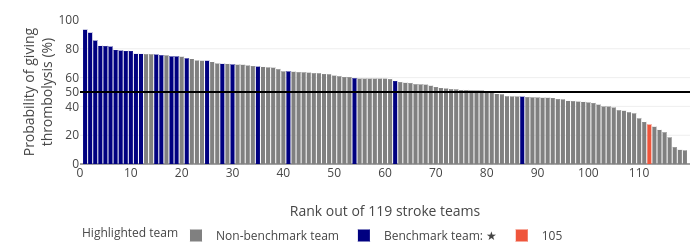
\includegraphics[width=1\textwidth]{./images/choice_example}
\end{center}

\vspace{2mm}
But who is right?!
\end{frame}
\begin{frame}
\frametitle{But would be the outcome for my patient?}

Machine learning allows personalised prediction of outcomes - so for that same patient, we can predict the probabilities of different levels of disability on discharge, with and without treatment.

\vspace{5mm}

\begin{center}
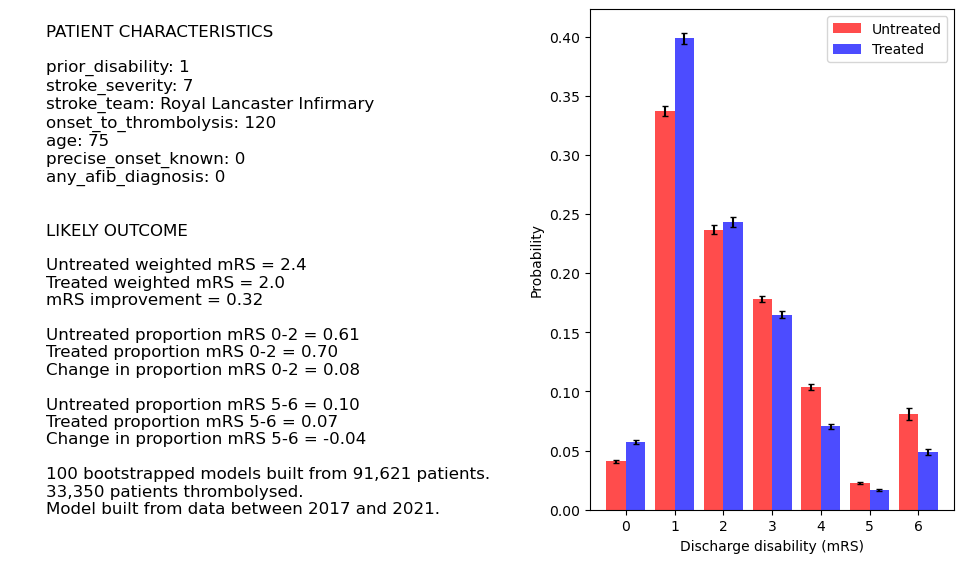
\includegraphics[width=0.8\textwidth]{./images/choice_example_outcome}
\end{center}


\end{frame}

\begin{frame}
\frametitle{With thanks especially to....}

\begin{itemize}
    \setlength{\itemsep}{2.mm}
    \item Our wonderful \textbf{Patient and Carer's Involvement team} (led by a former patient).
    \begin{itemize}
        \item To misquote Albert Einstein: `\textit{If you can't explain it to a public and patient involvement team, you don't understand it'}.
    \end{itemize}
    \item Our brilliant \textbf{qualitative research team} who are investigating how clinicians react to us using machine learning to analyse what they do differently (and how that affects outcomes).
    \item \textbf{Martin James}, who keeps asking difficult questions.
    \item \textbf{Anna Laws}, who has developed our web apps, while building mathematical models of outcomes, and writing clinical pathway simulation code.
    \item \textbf{Kerry Pearn}, who has developed our explainable machine learning work.
    
\end{itemize}

\end{frame}
\end{document}